\chapter{Introduction}
\label{cha:introduction}

\section{Research Background and Motivation}
\label{sec:introduction:background_motivation}

As industrial systems become more complex and automated under Industry 4.0, their reliability and safety are more critical than ever \cite{chen2017industry}. Unexpected equipment failures can lead to significant economic losses, production disruptions, and even safety accidents. Therefore, intelligent fault diagnosis technology, which can detect and identify potential faults in a timely and accurate manner, has become a key research area in industrial applications \cite{zhang2019deep, zhao2019deep}. Traditional fault diagnosis methods, which often rely on physical models or signal processing techniques combined with expert knowledge, struggle to cope with the massive, high-dimensional, and complex time-series data generated by modern sensor networks \cite{lei2016intelligent}. The data collected from industrial processes, such as vibration, pressure, and temperature signals, are often characterized by strong non-linearity and non-stationarity, making it difficult for these conventional methods to effectively extract discriminative fault features.

In recent years, data-driven approaches, particularly those based on deep learning, have shown great potential in overcoming these limitations \cite{liu2018artificial}. Deep learning models can automatically learn hierarchical features directly from raw sensor data, bypassing the need to manually design features, a process that is often slow and subjective \cite{khan2018review}. Among various deep learning architectures, Long Short-Term Memory (LSTM) networks, a specialized type of recurrent neural network (RNN), are particularly well-suited for modeling time-series data due to their ability to capture temporal dependencies \cite{hochreiter1997long}. LSTMs have been successfully applied to fault detection in industrial time series, demonstrating their effectiveness in learning from sequential patterns \cite{filonov2016multivariateindustrialtimeseries}. 

However, LSTMs process information sequentially, which can lead to challenges in capturing long-range dependencies in very long sequences and may suffer from computational inefficiency. More recently, the Transformer model, which relies entirely on a self-attention mechanism, has achieved state-of-the-art performance in various sequence modeling tasks \cite{vaswani2017attention}. The self-attention mechanism allows the Transformer to weigh the importance of all time steps simultaneously, enabling it to capture global dependencies and interactions within a sequence. This capability offers a new and powerful perspective for time-series analysis and has shown promise in fault diagnosis \cite{wen2021time}. Nevertheless, the standard Transformer architecture may not sufficiently capture the fine-grained, ordered nature of fault signatures as effectively as recurrent models.

This reveals a clear research gap: LSTMs excel at modeling local, sequential patterns but may miss critical long-range dependencies, while Transformers are adept at capturing global context but may overlook the nuanced, ordered progression inherent in fault evolution. The motivation for this thesis is that by combining the different strengths of these two architectures, it is possible to build a more effective model. This thesis hypothesizes that a hybrid model can achieve superior performance by leveraging the Transformer\'s ability to extract globally relevant features and then feeding these context-rich representations into an LSTM to model the temporal evolution of the system\'s health state. Furthermore, this research aims to address practical challenges such as class imbalance and multi-scale temporal patterns by proposing a novel hybrid Transformer-LSTM model that incorporates an adaptive fusion mechanism and a focal loss function, creating a fault diagnosis system that is both accurate and reliable.


\section{Analysis of Current Research Status}
\label{sec:introduction:current_status}

Fault diagnosis technology in the industrial sector has evolved through three main phases: physics-based models, traditional machine learning-based methods, and deep learning-based approaches \cite{lei2016intelligent, zhao2019deep}.

Early research primarily focused on physics-based models and signal processing techniques \cite{lei2020applications}. These methods attempt to build precise mathematical models for specific equipment or utilize techniques like Fourier Transform and Wavelet Transform to analyze signal characteristics in the time or frequency domain \cite{liu2018artificial}. However, these approaches often require extensive prior knowledge, involve complex model construction, and have limited generalization capabilities when faced with complex and variable operating conditions \cite{liu2018artificial}. Subsequently, traditional machine learning methods, represented by Support Vector Machines (SVM), k-Nearest Neighbors (k-NN), and Artificial Neural Networks (ANN), were introduced \cite{zhao2019deep}. While these methods improved the level of automation in diagnostics, their performance depended heavily on hand-crafted features. Designing these features is slow, difficult, and requires deep domain expertise, which prevented a fully automated diagnosis process \cite{lei2020applications, zhao2019deep}.

In recent years, data-driven methods, particularly those based on deep learning, have become the mainstream research direction in intelligent fault diagnosis due to their powerful capabilities in automatic feature extraction and non-linear modeling \cite{zhao2019deep, zhang2019deep, khan2018review}. Various deep learning models have been successfully applied \cite{lei2020applications, zhang2019deep}:

\begin{itemize}
    \item \textbf{Convolutional Neural Networks (CNN):} Initially achieving great success in image recognition, CNNs are now widely used to process one-dimensional signals like vibration and acoustic data, or their two-dimensional time-frequency representations \cite{zhang2019deep, liu2018artificial}. Through their unique convolutional and pooling operations, CNNs can effectively capture local correlations and translation-invariant features in signals, making them highly suitable for extracting discriminative fault patterns from industrial sensor data \cite{zhao2019deep, lei2020applications}.
    \item \textbf{Recurrent Neural Networks (RNN) and their variants:} RNNs, especially Long Short-Term Memory (LSTM) and Gated Recurrent Unit (GRU) networks, are specifically designed for processing sequential data \cite{hochreiter1997long}. They can effectively capture temporal dependencies, which is crucial for understanding the entire lifecycle of a fault from inception to evolution \cite{filonov2016multivariateindustrialtimeseries, khan2018review}. Nevertheless, these models may struggle to capture long-range dependencies in very long sequences due to issues like vanishing gradients \cite{pascanu2013difficulty}.
    \item \textbf{The Transformer Model:} To address the problem of long-range dependencies, the Transformer model, originally developed for natural language processing, was introduced to time-series analysis \cite{vaswani2017attention}. Its core self-attention mechanism allows for the parallel computation of dependencies between all elements in a sequence, enabling the direct capture of global information \cite{vaswani2017attention}. This has provided a new perspective for fault diagnosis, and studies have shown the great potential of Transformer-based models in time-series forecasting and classification tasks \cite{zhou2021informer, wen2021time}.
\end{itemize}

To combine the advantages of different models for superior performance, researchers have begun to explore hybrid deep learning models \cite{zhao2019deep, lei2020applications}. For instance, using a CNN to extract spatial features and then feeding the output to an LSTM for time-series modeling (CNN-LSTM) is a common and proven strategy \cite{khan2018review, zhao2019deep}. Similarly, attention mechanisms have been incorporated into traditional architectures to improve their ability to focus on relevant information \cite{bahdanau2015neural}. Recent studies have also explored the integration of different optimization techniques, such as adaptive learning rates \cite{kingma2014adam, loshchilov2019decoupled} and advanced regularization methods \cite{srivastava2014dropout}, to enhance model performance and robustness. The success of such combined models demonstrates that further improvements in diagnostic accuracy and robustness can be achieved by integrating the structural strengths of different architectures \cite{lei2020applications, khan2018review}. However, combining the Transformer's ability to see the "big picture" with the LSTM's skill in handling ordered sequences is still a new area of research. This gap presents a clear opportunity for the research in this thesis.




\section{Core Issues and Challenges}
\label{sec:introduction:issues_challenges}

Despite the progress in deep learning-based fault diagnosis, several core issues and challenges remain to be addressed to enhance the performance, robustness, and applicability of these models in real-world industrial settings. This thesis will focus on the following key challenges:

\subsection{Modeling of Long-Term Time-Dependent Relationships}
Industrial processes often exhibit complex temporal dynamics where the signature of a fault may evolve over a long period. Capturing these long-range dependencies is crucial for early and accurate diagnosis. While LSTMs are designed to model temporal sequences, they can struggle with very long sequences due to the risk of vanishing or exploding gradients \cite{pascanu2013difficulty}, making it difficult to relate current observations to events far in the past. The challenge lies in developing a model that can effectively bridge these long time lags and understand the complete temporal evolution of system behavior.

\subsection{Data Class Imbalance}
In real-world industrial applications, datasets for fault diagnosis are often highly imbalanced. Data for normal operating conditions are abundant, while data for specific fault types, especially critical or catastrophic failures, are scarce. This imbalance can severely bias a machine learning model, causing it to perform well on the majority class (normal operation) but poorly on the minority classes (faults). The challenge is to design a model and training strategy that can learn effectively from imbalanced data, for instance by using specialized sampling techniques \cite{chawla2002smote}, and accurately identify rare but critical fault events.

\subsection{Multi-Scale Time Pattern Analysis}
Fault signatures in time-series data can manifest at multiple time scales. For example, a gradual degradation process might be a long-term trend, while an intermittent fault could appear as a short-term, high-frequency burst. A robust diagnostic system must be capable of simultaneously analyzing and integrating information from these different time scales. Traditional models often focus on a single temporal resolution, potentially missing important patterns at other scales. The challenge is to develop an architecture that can effectively extract and fuse multi-scale temporal features \cite{zhang2019deep} to form a comprehensive understanding of the system's health state.

\begin{figure}[h!]
\centering
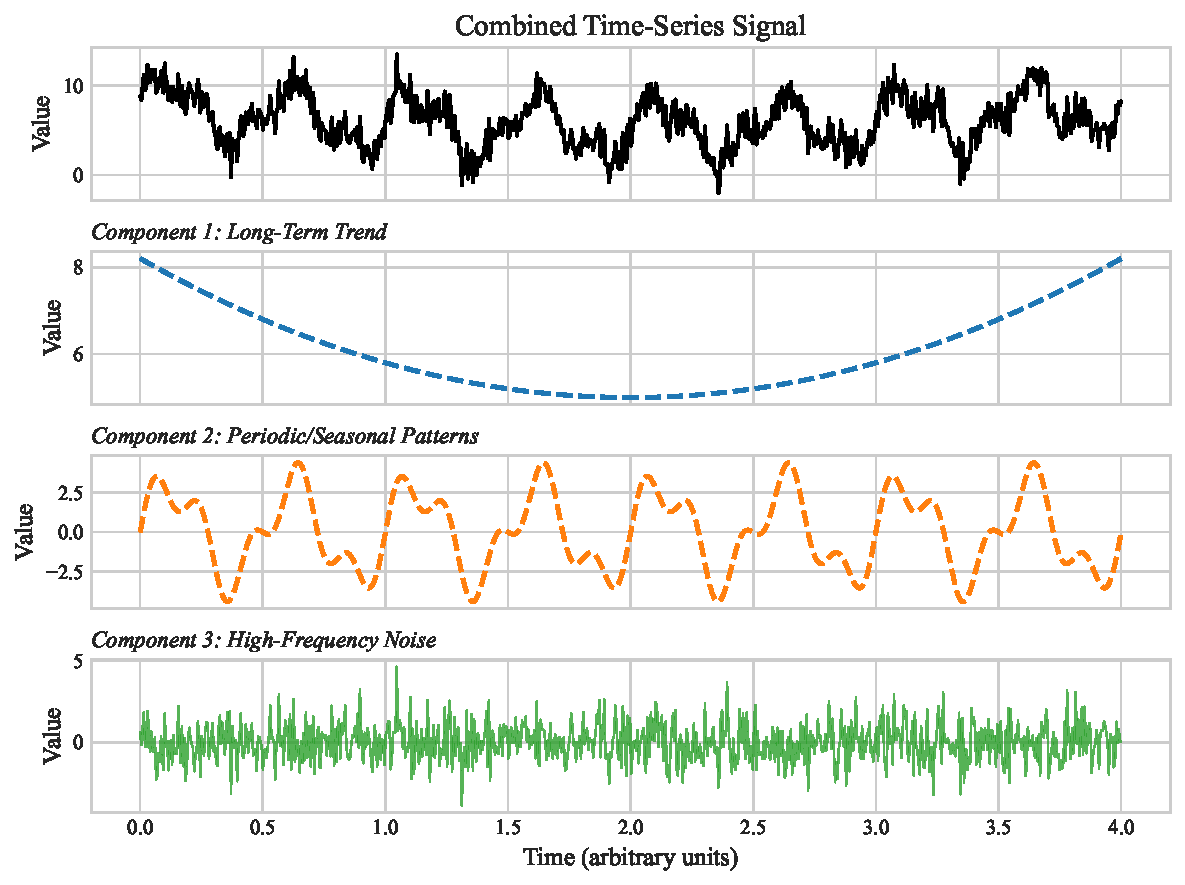
\includegraphics[width=0.8\textwidth]{logos/multi_scale_timeseries_decomposition.pdf}
\caption{An illustration of a complex time-series signal decomposed into its multi-scale components: a long-term trend, periodic patterns, and high-frequency noise.}
\label{fig:multi_scale_decomposition}
\end{figure}

\subsection{Generalization Ability to Different Working Conditions}
Industrial equipment often operates under various working conditions, such as different loads, speeds, or environmental factors. A fault diagnosis model trained on data from one set of conditions may not generalize well to others, as the fault signatures can vary significantly. This lack of generalization, often addressed with transfer learning techniques \cite{lei2020applications}, limits the practical deployment of diagnostic systems. The challenge is to build a model that is robust to variations in operating conditions and can extract invariant fault features, ensuring reliable performance across the full operational spectrum of the machinery.

\section{Main Research Content and Contributions}
\label{sec:introduction:content_contributions}

To address the challenges in industrial fault diagnosis, this thesis develops and tests a new hybrid deep learning system. The primary research content of this work is centered around building a hybrid architecture that combines Transformer and Long Short-Term Memory (LSTM) networks for better diagnostic performance. The key tasks undertaken in this research include:

Designing a Hybrid Transformer-LSTM Architecture: The main goal is to build a model that uses the unique strengths of both its parts. A Transformer encoder is employed to capture global dependencies and long-range correlations from multivariate sensor data, while a subsequent bidirectional LSTM (Bi-LSTM) network models the temporal evolution and sequential nature of the extracted features.

Developing an Adaptive Feature Fusion Strategy: A key part of the hybrid model is how it combines features from the Transformer and LSTM. This research proposes an adaptive fusion method that intelligently blends global context from the Transformer with local temporal patterns from the LSTM, helping the model focus on the most important information for diagnosis.

Addressing Real-World Challenges: This study also tackles practical issues commonly found in industrial environments, beyond just the core architecture. This includes utilizing a focal loss function to mitigate the effects of class imbalance, applying targeted data augmentation techniques for time-series data, and ensuring the model's robustness through appropriate regularization and training strategies.

Experimental Validation: The proposed model is thoroughly tested on a real industrial dataset with various fault types (e.g., backlash, baseline shift, jerk). Performance is compared against baseline models, including standalone Transformer and LSTM architectures, using detailed experiments and ablation studies.

The main contributions of this thesis, both theoretical and practical, are summarized as follows:

A New Hybrid Deep Learning Architecture for Fault Diagnosis: This thesis introduces a new hybrid model that successfully integrates Transformer and LSTM networks. This architecture offers a new way to analyze industrial time-series data. It models both global feature interactions and local temporal dynamics at the same time, overcoming a major limitation of using either model alone \cite{wen2021time}.

An Adaptive Fusion Mechanism for Better Feature Representation: This thesis proposes an adaptive fusion strategy that effectively combines features from different levels. Unlike simple concatenation, this mechanism allows the model to learn the optimal balance between global and sequential representations, leading to a more robust and discriminative feature space for classification.

A Complete Solution to Common Industrial Data Challenges: This research offers a comprehensive approach that tackles several practical problems at once. By integrating techniques like focal loss for class imbalance \cite{lin2017focal} and advanced regularization, this work provides a more complete and robust solution for real industrial applications.

Experimental Results and Practical Guidance for Industry: Through extensive experiments, this thesis shows that the proposed model performs better than conventional and single-architecture deep learning methods. The detailed methods and positive results offer practical guidance for implementing advanced AI-driven predictive maintenance systems in industrial settings.

\section{Thesis Chapter Organization}
\label{sec:introduction:organization}

The remainder of this thesis is structured as follows:

Chapter 2: Related Technologies and Theoretical Foundations provides a comprehensive review of the fundamental concepts underpinning this research. It covers the principles of Long Short-Term Memory (LSTM) networks, the architecture of the Transformer model, including the self-attention mechanism, and other key deep learning techniques relevant to this study.

Chapter 3: Fault Diagnosis Model based on Hybrid Transformer-LSTM details the proposed model. It presents the overall architecture, describes the data preprocessing pipeline, and elaborates on the design of the Transformer feature extraction component, the LSTM sequence modeling component, and the core adaptive feature fusion strategy.

Chapter 4: Experiments and Result Analysis describes the experimental setup, including the dataset, evaluation metrics, and hyperparameter settings. It presents a detailed analysis of the experimental results, including performance comparisons with baseline models, ablation studies to validate the contribution of each model component, and visualizations such as confusion matrices and learning curves.

Chapter 5: Conclusion and Future Work summarizes the key findings and and contributions of this research. It also discusses the limitations of the current work and suggests potential directions for future research, such as model optimization for real-time deployment and exploration of unsupervised learning methods.